% ==========================================================================
% Documento de Hallazgos — TechLogistics S.A.S.
% Informe de consultoría para la junta directiva
% Compilar con: pdflatex informe_hallazgos.tex  (dos pasadas)
% Las figuras en figuras/ se generan desde la app (src/eda.py + plotly)
% ==========================================================================
\documentclass[11pt,letterpaper]{article}

\usepackage[utf8]{inputenc}
\usepackage[T1]{fontenc}
\usepackage{lmodern}
\usepackage[margin=2.4cm]{geometry}
\usepackage{graphicx}
\usepackage{booktabs}
\usepackage{xcolor}
\usepackage{amsmath}
\usepackage[colorlinks=true, linkcolor=azuloscuro, urlcolor=azuloscuro]{hyperref}

% Paleta corporativa del informe (misma familia que el dashboard)
\definecolor{azuloscuro}{HTML}{1A5276}
\definecolor{rojoalerta}{HTML}{C0392B}
\definecolor{verdeok}{HTML}{1E8449}
\definecolor{grisclaro}{HTML}{F2F3F4}

\setlength{\parskip}{6pt}
\setlength{\parindent}{0pt}

% Cajita simple para los mensajes clave de cada sección
\newcommand{\mensajeclave}[1]{%
  \vspace{4pt}
  \noindent\colorbox{grisclaro}{\parbox{\dimexpr\linewidth-2\fboxsep}{%
    \textbf{\textcolor{azuloscuro}{Mensaje para la junta:}} #1}}
  \vspace{4pt}
}

\begin{document}

% ------------------------------- Portada ---------------------------------
\begin{titlepage}
  \centering
  \vspace*{2cm}
  {\color{azuloscuro}\rule{\linewidth}{2pt}}\\[1.2cm]
  {\Huge\bfseries\color{azuloscuro} Documento de Hallazgos}\\[0.5cm]
  {\Large Del Caos al Storytelling: auditoría e inteligencia\\ sobre los tres sistemas de TechLogistics S.A.S.}\\[1.2cm]
  {\color{azuloscuro}\rule{\linewidth}{2pt}}\\[2cm]
  {\large\textbf{Informe de consultoría dirigido a la Junta Directiva}}\\[1.5cm]
  {\large\textbf{Equipo consultor}}\\[0.3cm]
  {\large Miguel Ángel Cano Salinas}\\
  {\large Daniel Correa Botero}\\
  {\large Daniel Felipe Arango Guarín}\\[1.8cm]
  \begin{tabular}{ll}
    \textbf{Cliente:} & TechLogistics S.A.S.\\
    \textbf{Alcance:} & Inventario ERP, Logística y Feedback de clientes\\
    \textbf{Registros auditados:} & 17.000 (2.500 + 10.000 + 4.500)\\
    \textbf{Herramientas:} & Python · Pandas · Streamlit · Plotly · Groq (Llama-3)\\
    \textbf{Fecha:} & Julio de 2026\\
  \end{tabular}
  \vfill
\end{titlepage}

% --------------------------- Resumen ejecutivo -----------------------------
\section*{Resumen ejecutivo}

La junta sospechaba de una \emph{invisibilidad operativa} entre sus tres
sistemas. La auditoría lo confirma y le pone cifras: sobre un ingreso total de
\textbf{\$74,6 millones USD}, la compañía pierde \textbf{\$7,6 millones} en 879
productos que se venden por debajo de su costo, y otros \textbf{\$13,0 millones
(17,4\% del ingreso)} fluyen por 480 referencias que no existen en el maestro
de inventario. A esto se suma una operación logística uniformemente lenta
(15 días promedio de entrega) y bodegas que llevan más de un año sin conteo
físico, con tasas de reclamo cercanas al 50\%.

La buena noticia: ninguno de estos problemas es invisible una vez los sistemas
hablan entre sí. Este informe documenta la limpieza aplicada (con su
justificación ética), responde las cinco preguntas estratégicas planteadas y
cierra con un plan de acción priorizado.

\section{Auditoría de calidad: el punto de partida}

Ningún dato se transformó sin dejar rastro. Cada dataset recibió un
\emph{Health Score} (40\% completitud, 20\% unicidad, 40\% validez de negocio)
antes y después del procesamiento; la bitácora completa de decisiones es
descargable desde la aplicación.

\begin{figure}[h!]
  \centering
  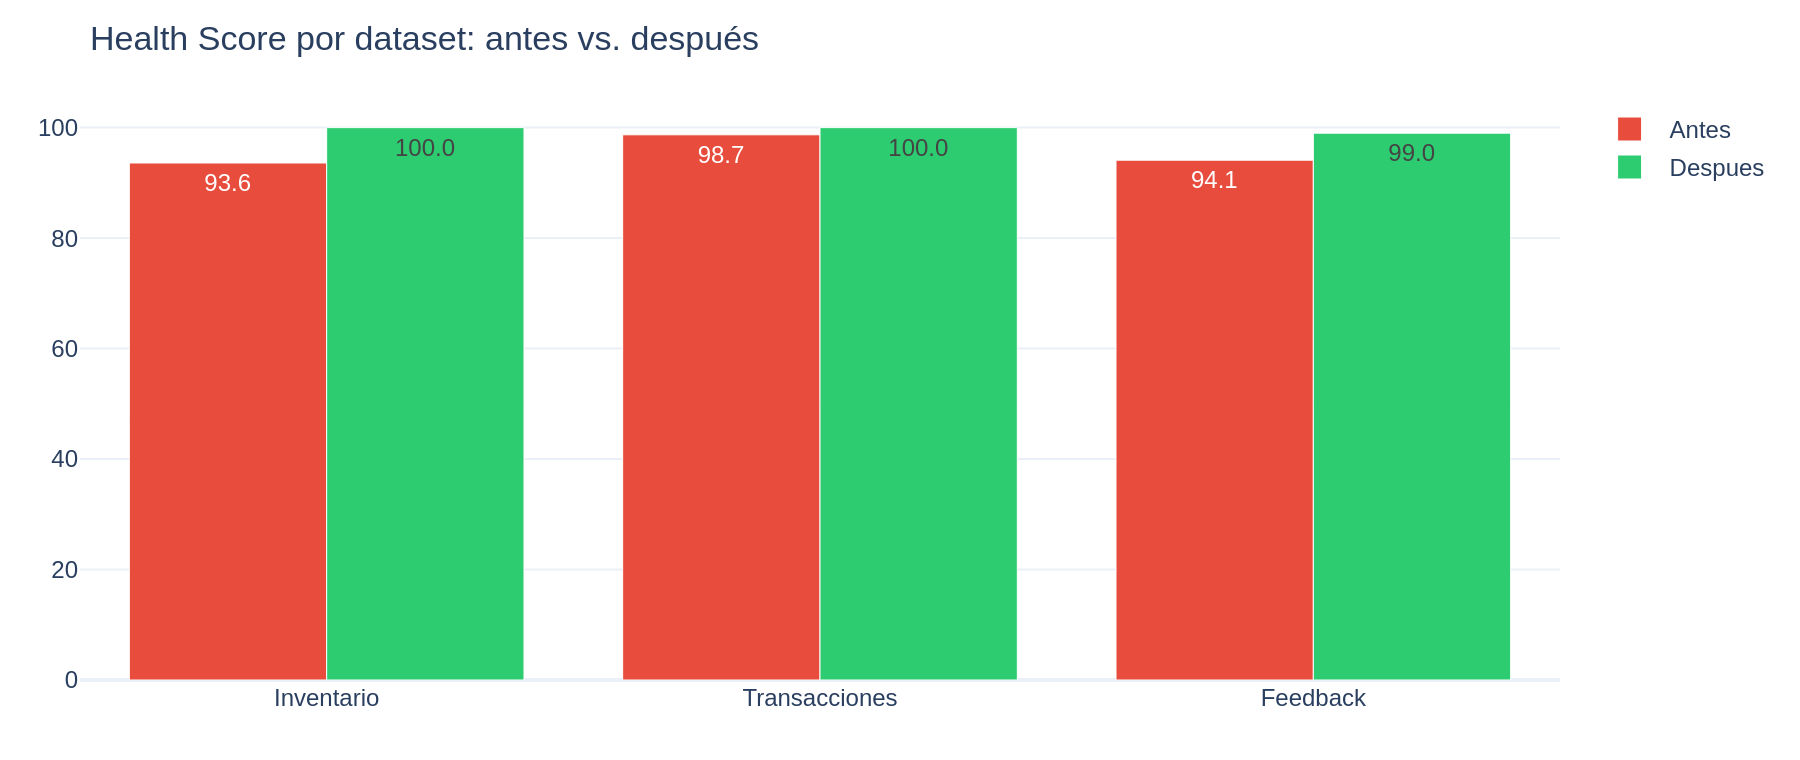
\includegraphics[width=0.82\textwidth]{figuras/health_score.png}
  \caption{Health Score por dataset. Inventario pasó de 93,6 a 100; transacciones de 98,7 a 100; feedback de 94,1 a 99,0.}
\end{figure}

Las intervenciones más relevantes, con su justificación:

\begin{itemize}
  \item \textbf{Imputación con mediana} para costos fuera de rango
        (\$0,05--\$850.000), stock nulo, edades imposibles (hasta 195 años) y
        tiempos de entrega con el centinela 999: la mediana no se deja
        arrastrar por los mismos extremos que se están corrigiendo.
  \item \textbf{Imputación con moda} para el rating 99 en una escala 1--5,
        por tratarse de una variable ordinal discreta.
  \item \textbf{Sin imputación} donde la ausencia es información: los estados
        de envío nulos se etiquetaron como ``Sin Registro'' en lugar de
        asignarles la moda, que falsearía el seguimiento de última milla.
  \item \textbf{Eliminación mínima}: solo se excluyeron las 100 transacciones
        con cantidad negativa (devoluciones, 1\% del total) y los 877
        registros de feedback duplicados por transacción, que inflaban el
        peso de algunos clientes en el NPS.
\end{itemize}

% ------------------------------ Pregunta 1 ---------------------------------
\section{Fuga de capital: productos que destruyen valor}

\textbf{879 SKUs se venden con margen negativo}, acumulando una pérdida de
\textbf{\$7,59 millones USD}. El caso extremo, PROD-2858 (Smartphones), pierde
\$57.239 con solo 8 transacciones: prácticamente devuelve en pérdida todo lo
que factura.

\begin{figure}[h!]
  \centering
  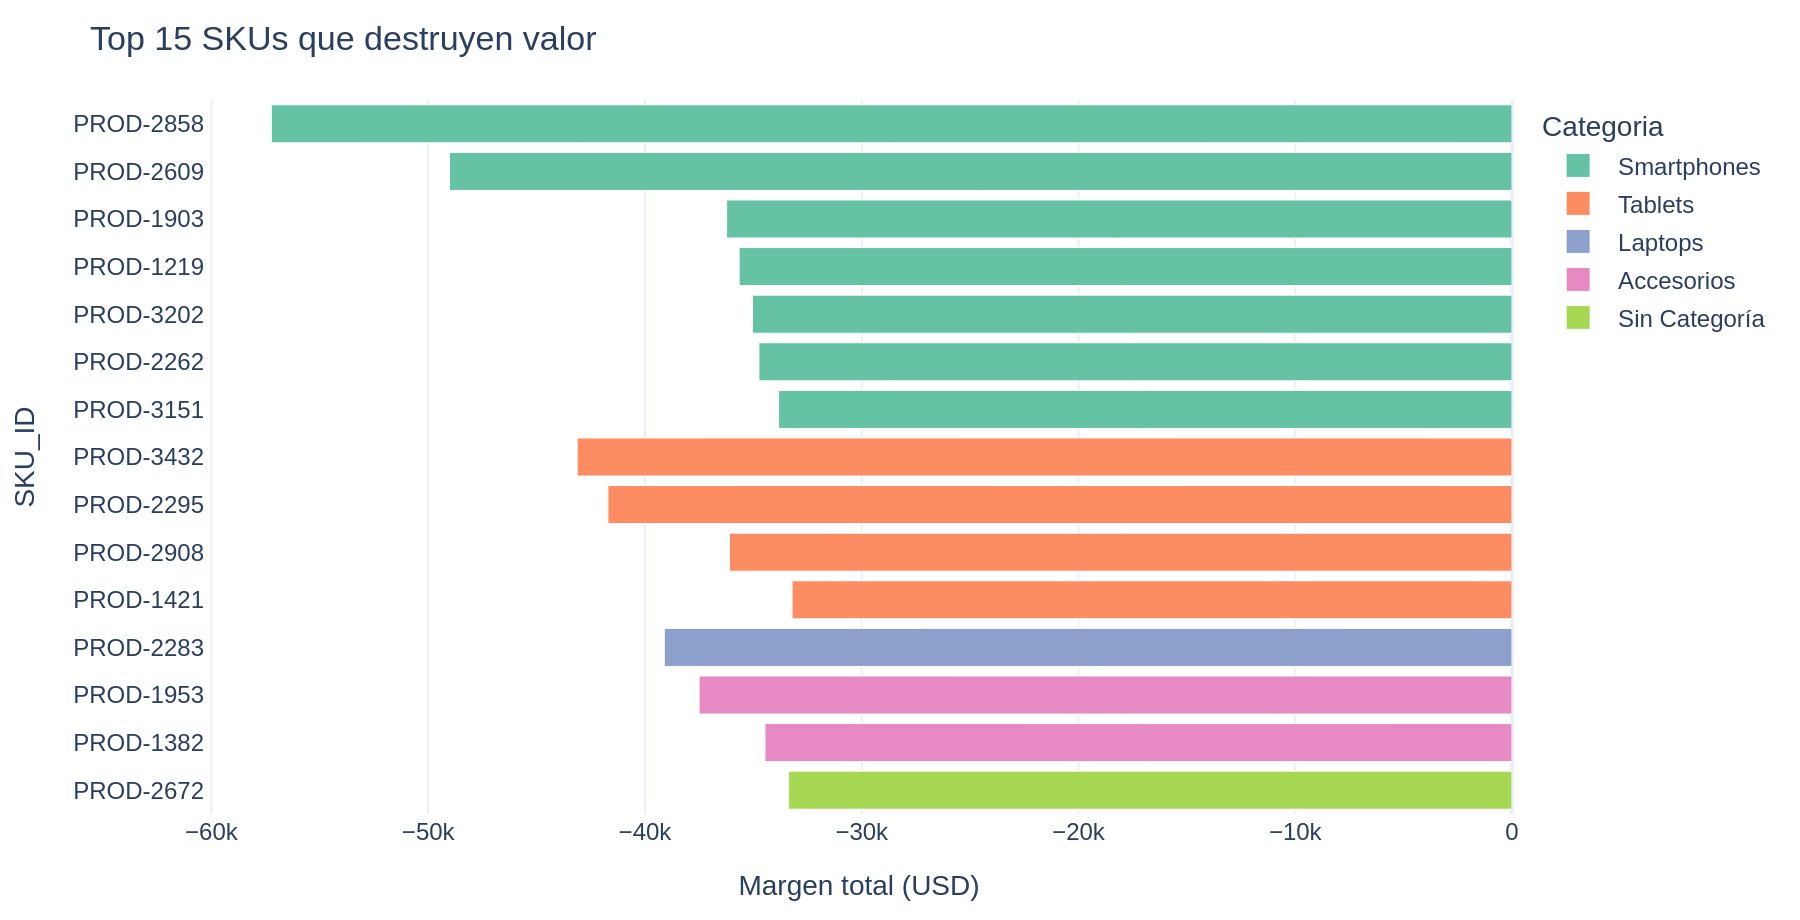
\includegraphics[width=0.9\textwidth]{figuras/p1_skus_negativos.png}
  \caption{Los 15 SKUs con mayor destrucción de valor, coloreados por categoría.}
\end{figure}

¿Es una falla del canal Online, como se temía? No. La pérdida se reparte de
forma casi pareja: Físico (\$3,09M), WhatsApp (\$3,02M), Online (\$2,79M) y App
(\$2,65M).

\begin{figure}[h!]
  \centering
  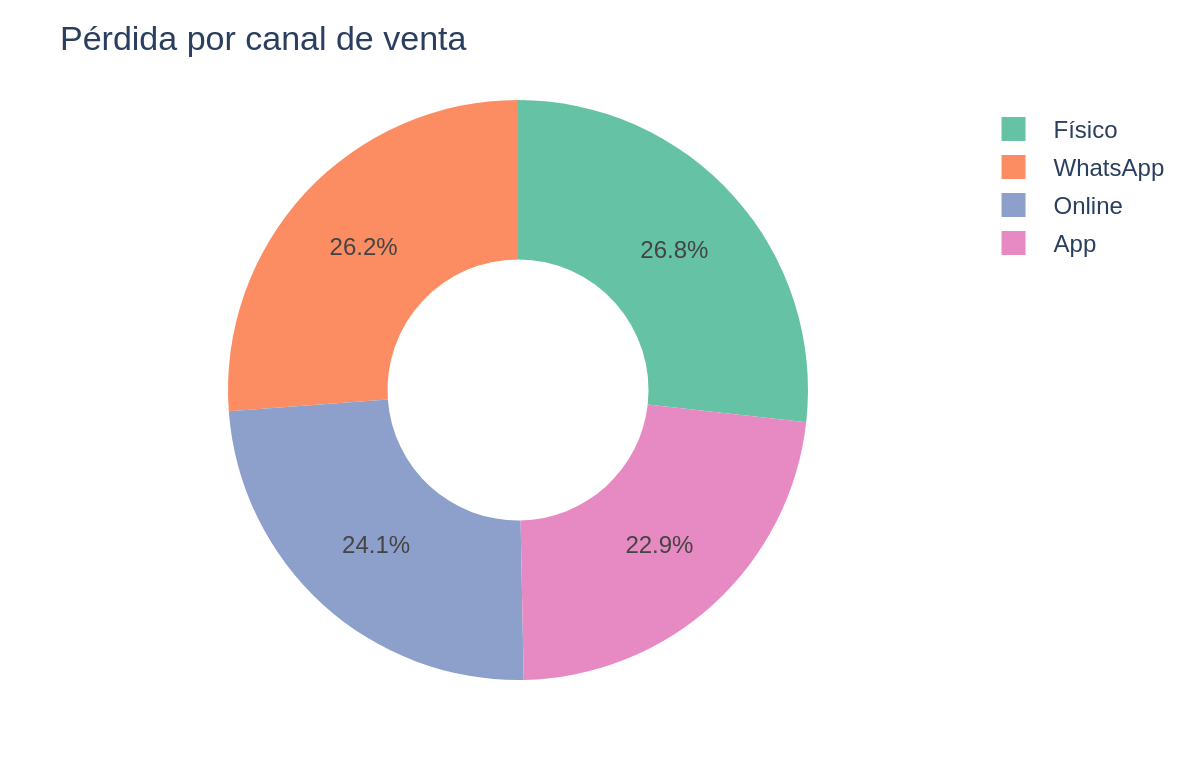
\includegraphics[width=0.5\textwidth]{figuras/p1_perdida_canal.png}
  \caption{Distribución de la pérdida por canal: ningún canal concentra el problema.}
\end{figure}

\mensajeclave{La fuga no es una guerra de precios de un canal: es una falla
estructural de \emph{pricing} por producto (costos mal cargados o descuentos
sin piso). Se recomienda un piso de precio automático: ninguna orden puede
salir por debajo del costo unitario más el flete sin aprobación gerencial.}

% ------------------------------ Pregunta 2 ---------------------------------
\section{Crisis logística: ¿dónde duele más cada día de retraso?}

Aquí el hallazgo honesto es que \textbf{la correlación entrega--NPS es débil en
todas las zonas} (entre $-0{,}03$ y $+0{,}04$): no existe una ciudad
``verdugo'' que explique la caída de lealtad. La razón es incómoda: la
lentitud es \emph{uniforme}. Todas las ciudades promedian 13,7--15,7 días de
entrega, de modo que el castigo del cliente no discrimina por geografía.

\begin{figure}[h!]
  \centering
  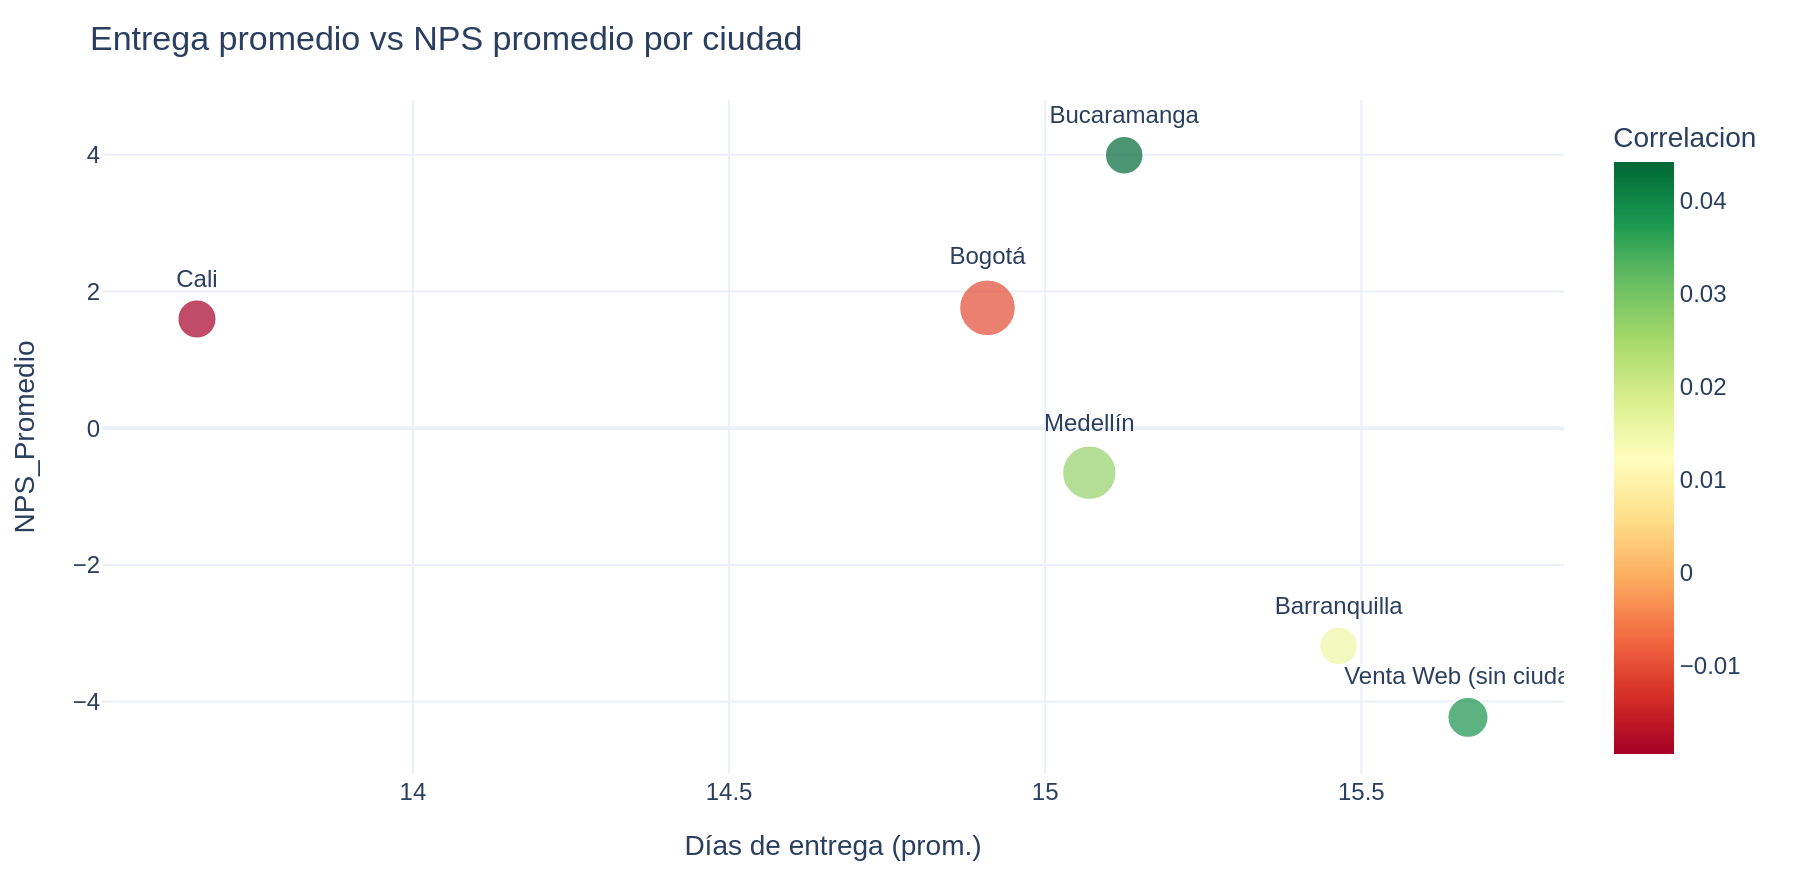
\includegraphics[width=0.88\textwidth]{figuras/p2_entrega_nps.png}
  \caption{Entrega promedio vs.\ NPS por ciudad. El tamaño indica volumen de muestras.}
\end{figure}

Aun así, hay prioridades claras: \textbf{Venta Web (sin ciudad)} combina la
entrega más lenta (15,7 días) con el peor NPS ($-4{,}2$), y
\textbf{Barranquilla} le sigue con 15,5 días y NPS $-3{,}2$. Por bodega,
\textbf{Zona Franca} presenta la correlación más negativa y el peor NPS
($-3{,}6$).

\mensajeclave{Más que cambiar un operador puntual, la meta debe ser bajar el
promedio general de 15 a menos de 8 días. Como primeros pilotos: el flujo de
Venta Web (que además viaja sin ciudad registrada, otro fallo de captura) y
la operación de Zona Franca.}

% ------------------------------ Pregunta 3 ---------------------------------
\section{La venta invisible: el hueco de \$13 millones}

De las 9.900 ventas válidas, \textbf{1.728 (17,5\%) corresponden a 480 SKUs que
no existen en el maestro de inventario}: las llamadas \emph{ventas fantasma}.
Representan \textbf{\$12,98 millones USD, el 17,4\% del ingreso total}, dinero
real que hoy fluye sin control de stock, costo ni margen.

\begin{figure}[h!]
  \centering
  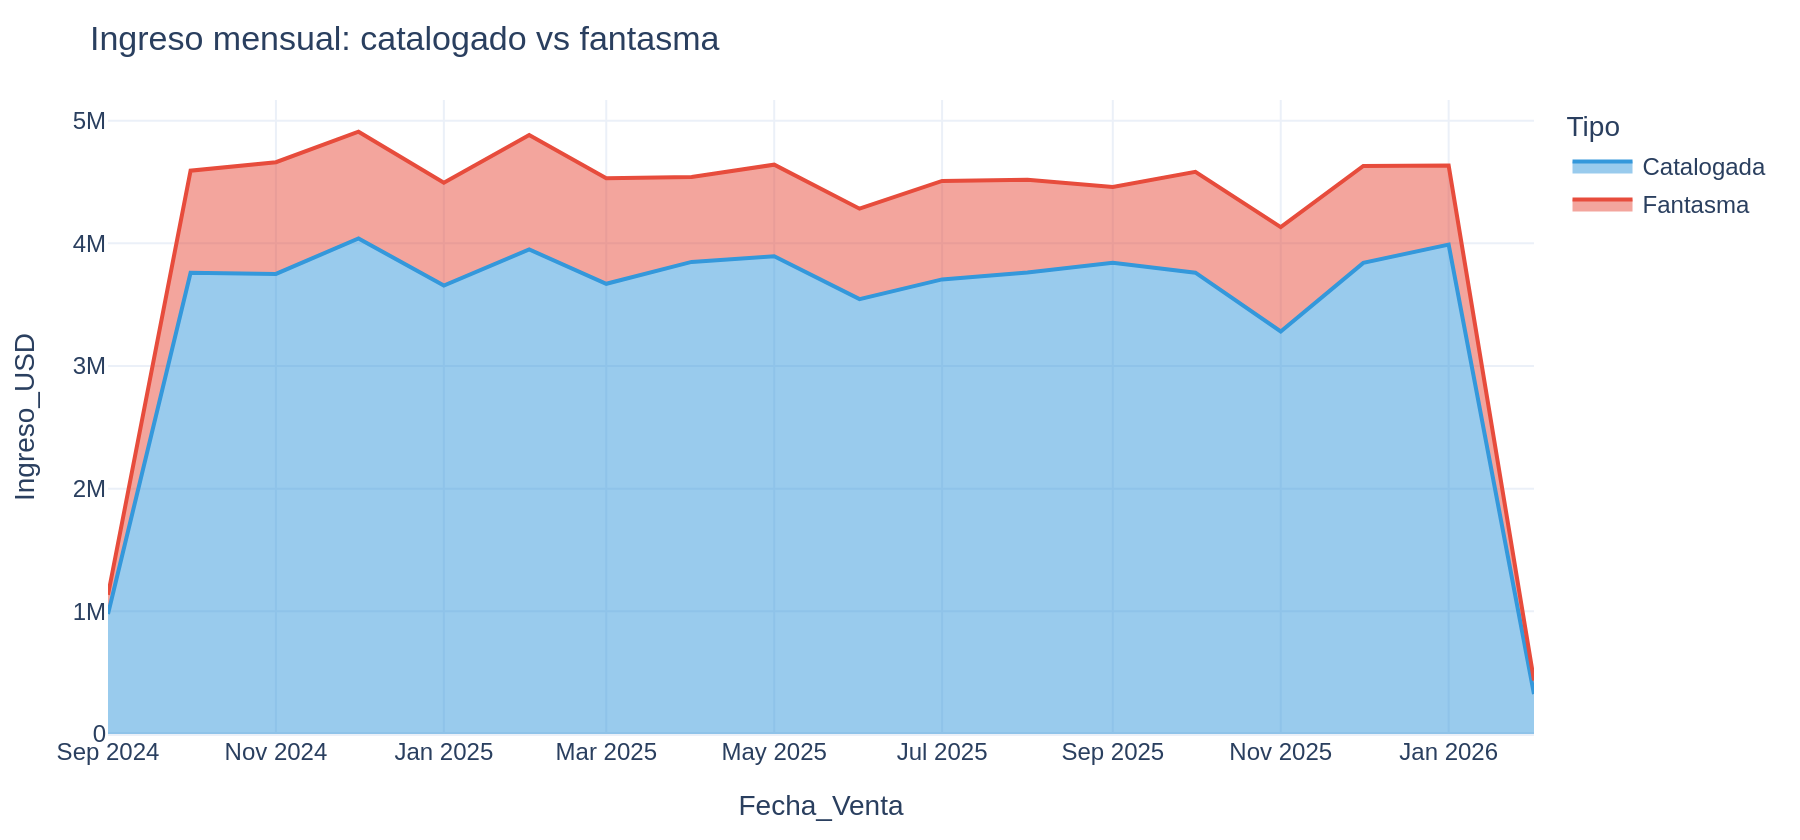
\includegraphics[width=0.9\textwidth]{figuras/p3_fantasma_mensual.png}
  \caption{Ingreso mensual catalogado vs.\ fantasma: el fenómeno es constante en todo el periodo.}
\end{figure}

\textbf{Diagnóstico: falla de catálogo, no fraude.} Tres evidencias lo
sustentan: el fenómeno aparece en los cuatro canales por igual, se mantiene
estable durante todo el periodo, y los SKUs siguen el mismo formato de
codificación del maestro (serie PROD-3xxx, consecutiva a la catalogada). Un
fraude tendría concentración por canal, bodega o fecha; esto parece la firma
de productos nuevos vendidos antes de sincronizar el ERP.

\mensajeclave{Decisión aplicada en el análisis: estas ventas se conservan como
ingreso (el dinero entró) pero se excluyen del cálculo de margen, porque
inventar un costo sería maquillar el estado de resultados. Acción: conciliación
de catálogo entre el ERP y los canales de venta, con bloqueo de facturación
para SKUs no registrados.}

% ------------------------------ Pregunta 4 ---------------------------------
\section{Paradoja de fidelidad: bodegas llenas, clientes molestos}

\textbf{Smartphones} es la categoría en paradoja: tiene el stock promedio más
alto (1.020 unidades) y a la vez el peor sentimiento (NPS $-5{,}0$), con el
mayor volumen de ventas (2.051 transacciones).

\begin{figure}[h!]
  \centering
  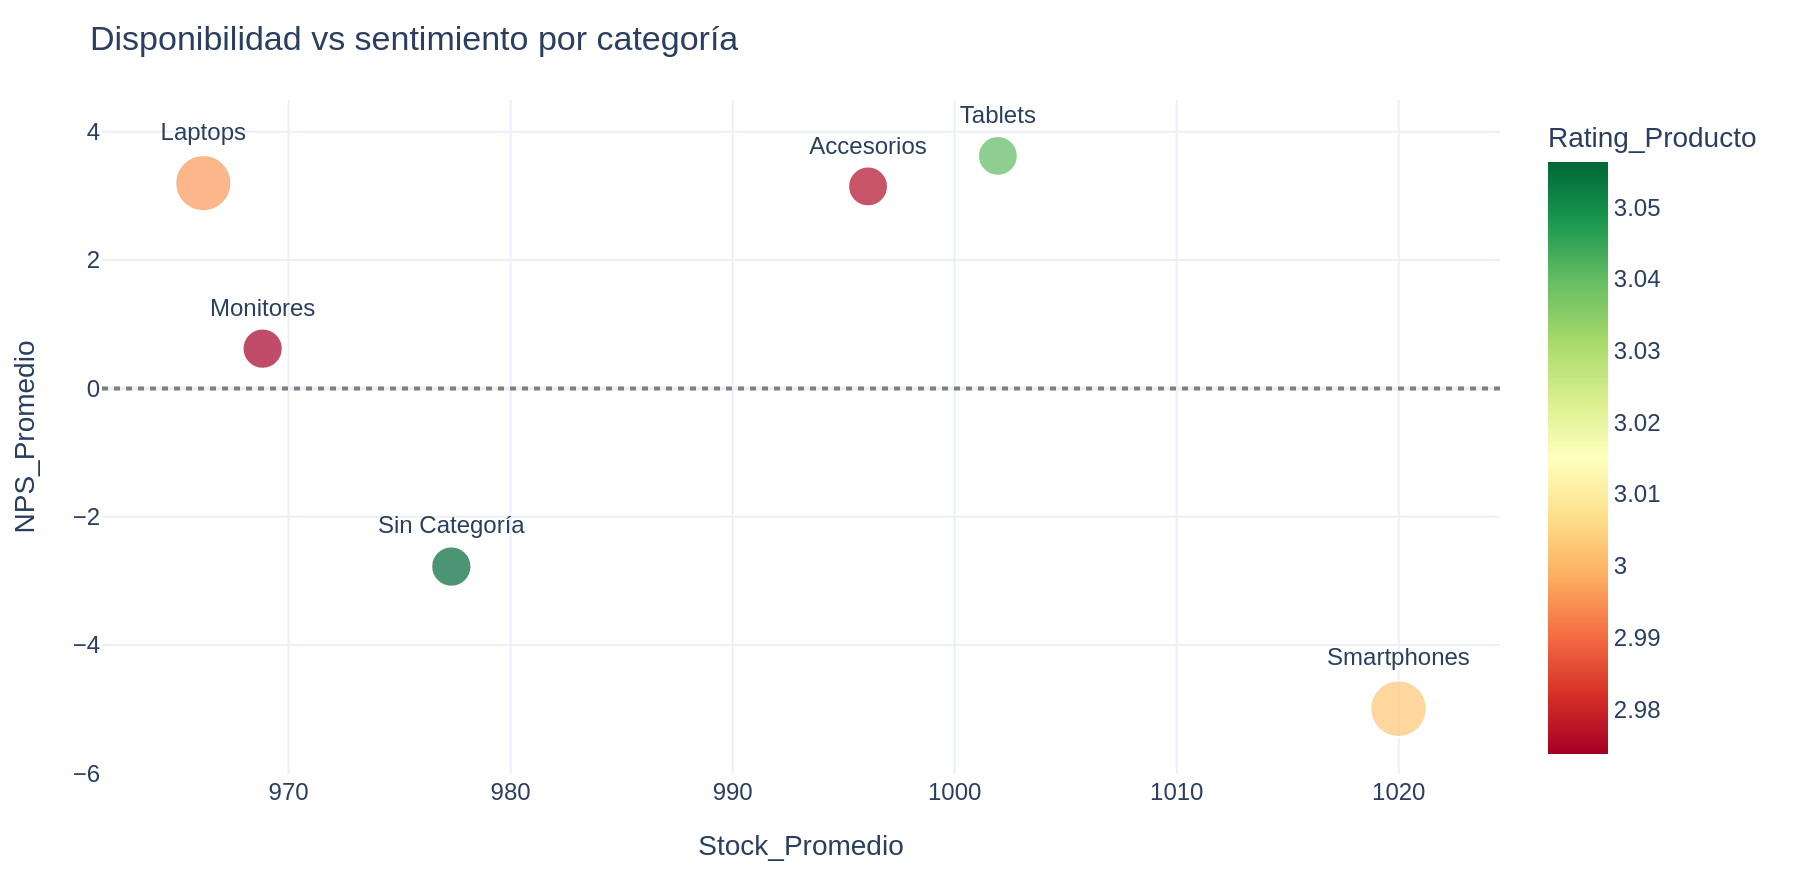
\includegraphics[width=0.88\textwidth]{figuras/p4_paradoja.png}
  \caption{Disponibilidad vs.\ sentimiento. Smartphones: mucho stock, NPS negativo.}
\end{figure}

¿Mala calidad o sobrecosto? Los datos apuntan a \textbf{sobrecosto}: el rating
de producto de Smartphones (3,0) es idéntico al del resto de categorías, es
decir, el producto no es peor. Lo que sí es distinto es su costo unitario
promedio (\$790, el más alto del portafolio) frente a un precio de venta
similar al de las demás (\$1.010). El cliente percibe que paga más sin recibir
más, y lo cobra en la recomendación.

\mensajeclave{No es un problema de fábrica sino de propuesta de valor:
renegociar costo con el proveedor de Smartphones o reposicionar el precio.
Mientras tanto, el sobre-stock de esta categoría es capital inmovilizado en
el producto que menos lealtad genera.}

% ------------------------------ Pregunta 5 ---------------------------------
\section{Riesgo operativo: bodegas que operan a ciegas}

El hallazgo más estructural: \textbf{las cinco bodegas llevan en promedio
más de un año (357--384 días) sin conteo físico de inventario}, y en todas
ellas prácticamente una de cada dos ventas termina en ticket de soporte
(48--53\%).

\begin{figure}[h!]
  \centering
  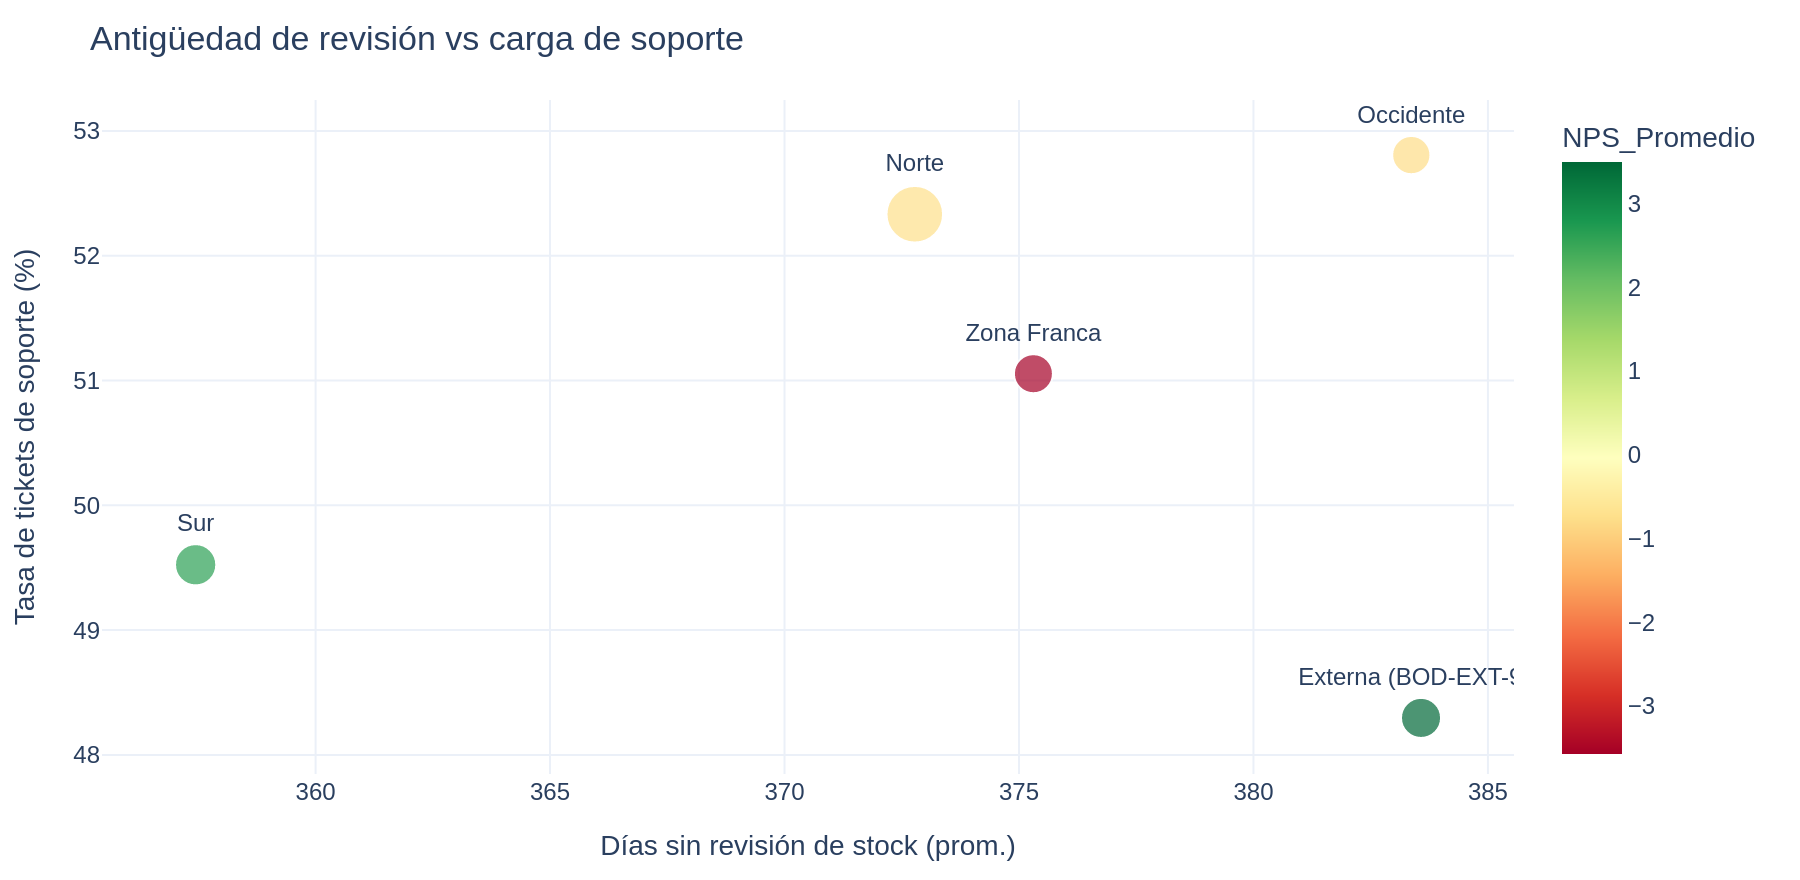
\includegraphics[width=0.88\textwidth]{figuras/p5_riesgo_bodegas.png}
  \caption{Antigüedad del último conteo vs.\ tasa de tickets por bodega.}
\end{figure}

\begin{table}[h!]
  \centering
  \small
  \begin{tabular}{lrrr}
    \toprule
    \textbf{Bodega} & \textbf{Días sin revisión} & \textbf{Tickets (\%)} & \textbf{NPS} \\
    \midrule
    Externa (BOD-EXT-99) & 384 & 48,3 & $+3{,}5$ \\
    Occidente            & 383 & 52,8 & $-0{,}8$ \\
    Zona Franca          & 375 & 51,1 & $-3{,}6$ \\
    Norte                & 373 & 52,3 & $-0{,}7$ \\
    Sur                  & 357 & 49,5 & $+2{,}6$ \\
    \bottomrule
  \end{tabular}
  \caption{Las bodegas más críticas combinan revisiones viejas, alta carga de soporte y NPS negativo.}
\end{table}

\textbf{Occidente} y \textbf{Zona Franca} son las que operan más a ciegas en
términos combinados: revisiones de más de un año, las tasas de reclamo más
altas y NPS negativo. Un stock que nadie verifica termina prometiendo unidades
que no existen; esa promesa rota se paga dos veces, en soporte y en lealtad.

\mensajeclave{Instaurar conteos cíclicos trimestrales obligatorios, empezando
por Occidente y Zona Franca. El dato de inventario es la materia prima de la
promesa de entrega: si está vencido, todo lo demás falla en cadena.}

% ------------------------------ Cierre --------------------------------------
\section{Plan de acción priorizado}

\begin{enumerate}
  \item \textbf{Inmediato (0--30 días):} piso de precio automático sobre
        costo + flete (frena la fuga de \$7,6M) y bloqueo de facturación para
        SKUs fuera de catálogo (controla el 17,4\% del ingreso en riesgo).
  \item \textbf{Corto plazo (30--90 días):} conciliación completa del maestro
        de productos con los canales; conteo físico en Occidente y Zona
        Franca; piloto logístico en el flujo de Venta Web.
  \item \textbf{Mediano plazo (90--180 días):} renegociación del costo de
        Smartphones o reposicionamiento de precio; meta de entrega menor a
        8 días; conteos cíclicos trimestrales institucionalizados.
\end{enumerate}

Todas las cifras de este documento son reproducibles: la aplicación Streamlit
que acompaña este repositorio permite filtrar por categoría, ciudad, canal y
fecha, regenerar cada gráfica y descargar la bitácora completa de limpieza.

\vspace{1em}
\begin{center}
  \color{azuloscuro}\rule{0.6\linewidth}{1pt}\\[0.5em]
  \small Miguel Ángel Cano Salinas · Daniel Correa Botero · Daniel Felipe Arango Guarín
\end{center}

\end{document}
